%% Introduction
\chapter{Introducción}\label{chap:intro}
\section{Propósito}\label{sec:purpose}
El propósito de este documento es múltiple: por una parte, el de establecer
un punto de partida claro y conciso en el desarrollo del proyecto. Una correcta
especificación acompañada de sus correspondientes diagramas y estructuración
permite iniciar el diseño, desarrollo y verificación del proyecto con ideas
claras y evaluadas con anterioridad, afrontando los posibles fallos o problemas
que puedan surgir y previendo situaciones complejas o errores en el diseño.

Por otra parte, el documento se redacta como especificación formal de
requisitos de usuario, funcionales, no funcionales, restricciones en el
desarrollo, requisitos de interfaces externas y de entorno físico del proyecto.
Esto sirve como ``contrato'' con aquello que debe aparecer y existir en
una implementación final del proyecto (\textit{requisitos funcionales}),
otros requisitos que son importantes pero que, en un momento dado, no aportan
funcionalidad al producto (\textit{requisitos no funcionales}), las
características de los usuarios que quieran usar el producto y otras restricciones
o información relevante que se haya de tener en cuenta a la hora de diseñar, 
desarrollar y probar el producto antes de darlo por concluido.

Finalmente, este documento se redacta orientado a otros ingenieros que
tengan curiosidad o interés en cómo se ha desarrollado el proyecto, las necesidades
que se han de suplir, qué características conforman el producto final o mismamente
replicar el proyecto para hacer una implementación propia o añadir alguna 
característica nueva. Sin embargo, con intención de facilitar la accesibilidad del
documento, se buscará ser claro y conciso en la especificación, usando un
lenguaje formal que sea preciso. Por ello, se incluye un apartado de definiciones,
acrónimos y abreviaturas (sección \ref{sec:definitions}) que pretenden servir
de orientación en el lenguaje técnico que se usará en el documento.
\section{Alcance}\label{sec:aim}
El objetivo principal de este \ac{PFM} es el de diseñar un sistema de recolección
de métricas orientado a vehículos en el ámbito del \ac{IoT} (\ac{VIMS}, de ahora en adelante)
que permita, utilizando los conectores estándar del vehículo, generar y almacenar
información relevante del vehículo, la conducción y demás factores de interés que
se den mientras se interactúa con el vehículo.

El sistema \ac{VIMS} deberá poder conectarse a Internet desde cualquier punto
geográfico\footnote{Dentro de las restricciones y limitaciones físicas y 
geográficas del entorno.} usando el automóvil como sistema de alimentación y
fuente de información. De esta manera, podrá enviar todo tipo de datos provistos 
a un servidor en donde se gestionarán, almacenarán y procesarán para 
una posterior visualización y generación de información.

Además, el sistema deberá poder integrarse con cualquier vehículo del mercado que
utilice las conexiones estándar reguladas y que trabaje con tramas e información
estandarizada. En otro caso, el sistema no funcionará correctamente y puede
comportarse de manera impredecible.

La infraestructura del servidor por su parte deberá poder recibir una gran cantidad
de datos (según estimaciones del mundo \ac{IoT}, se pueden recibir del orden de
varios \ac{GB} diarios \cite{vishHowMuchData2020}) y gestionarlos debidamente.
Cada dispositivo emisor se considerará único, por lo que los datos recibidos
deberán ser clasificados acorde a quién los emite.

Sin embargo, el sistema no modificará parámetros del vehículo ni realizará
modificaciones sobre la configuración del mismo: se limitará a ser un ``espía''
y no emitirá ningún dato hacia el automóvil.

Finalmente, desde el propio vehículo con un dispositivo externo (como un
\textit{smartphone}) se podrán acceder a los datos en tiempo real que ofrece el
vehículo mediante una interfaz hacia el sistema \ac{VIMS}. De esta manera, se
podrá saber rápidamente el estado del automóvil y detectar fallos en el mismo.

Así, el producto está orientado para su implantación en cualquier vehículo y que,
haciendo uso de las características de conectividad inalámbrica que presentará, pueda
adaptarse a nuevos automóviles y nuevas tramas estándar. Su venta está dirigida
principalmente a conductores que cuenten con un vehículo con algún conector estándar
compatible.

Este documento sigue la taxonomía de especificación descrita en la sección anterior (\ref{sec:purpose})
y abraca una actividad adicional que consistirá en una validación de los requisitos,
definida en el anexo \ref{chap:validation}.
\section{Definiciones, acrónimos y abreviaturas}\label{sec:definitions}
\begin{acronym}
  \acro{GB}{\textit{gigabyte}}
  \acro{IoT}{\textit{Internet of Things}}
  \acro{PFM}{Proyecto Fin de Máster}
  \acro{VIMS}{\textit{Vehicle IoT Metrics System}}
  \acro{OBD}{\textit{On-Borad Diagnostics}}
  \acro{GPS}{\textit{Global Positioning System}}
  \acro{BLE}{\textit{Bluetooth Low Energy}}
  \acro{PAN}{\textit{Personal Area Network}}
  \acro{CAN}{\textit{Controller Area Network}}
  \acro{API}{\textit{Application Programming Interface}}
  \acro{PAN}{\textit{Personal Area Network}}
\end{acronym}

\begin{itemize}
  \item \ac{GB} -- unidad de almacenamiento de información equivalente a $10^9$ bytes.
  \item \ac{IoT} -- concepto que se refiere a la interconexión digital de objetos 
        cotidianos con Internet \cite{InternetCosas2021}.
  \item \ac{OBD} -- sistema de diagnóstico a bordo de vehículos que
        cuenta con múltiples estándares según la región de uso. Estos
        sistemas ofrecen una monitorización activa y control completo
        sobre el motor y otros dispositivos del vehículo \cite{OBD2021}.
  \item \textit{jitter} -- retardo relativo que se produce en las comunicaciones
        y que afecta directamente a la saturación de la red y a la capacidad de
        transmisión de la misma.
  \item \ac{GPS} -- sistema que permite posicionar cualquier objeto con una 
        precisión de hasta centímetros usando cuatro o más satélites y 
        trilateración \cite{GPS2021}.
  \item trilateración -- método matemático que permite determinar las posiciones
        relativas de objetos usando la geometría de los triángulos \cite{Trilateracion2021}.
  \item \ac{BLE} -- tecnología \ac{PAN} que permite la comunicación entre dispositivos
        con un rango similar a Bluetooth pero un menor consumo de energía.
  \item Bus \ac{CAN} -- protocolo de comunicaciones para el envío de
        mensajes en entornos distribuidos, permitiendo la comunicación
        entre múltiples CPUs.
  \item \ac{API} -- conjunto de definiciones, subrutinas y protocolos que ofrecen
        ciertos \textit{softwares} para ser usados por otras aplicaciones como
        capa de abstracción sobre el original \cite{InterfazProgramacionAplicaciones2021}.
  \item \ac{PAN} -- redes destinadas a la comunicación entre dispositivos en una
        misma red o malla. Tiene un alcance muy limitado, de unos pocos metros por
        lo general.
\end{itemize}
\section{Estructura del documento}\label{sec:structure}

%% Product description
\chapter{Descripción general del producto}\label{chap:description}
A lo largo de esta sección se va a presentar el producto en sí, presentando por una
parte la perspectiva del mismo (\ref{ssec:perspective}), las características de
los usuarios finales (\ref{ssec:specs}), restricciones generales que se aplican sobre
el producto (\ref{ssec:restrictions}) y supuestos y dependencias sobre el proyecto
que afectan directamente al desarrollo (\ref{ssec:dependencies}).
\section{Perspectiva del producto}\label{sec:perspective}
\ac{VIMS} se constituirá de un módulo independiente diseñado desde cero aprovechando
las tecnologías que ofrecen los vehículos de forma estándar (como el conector
\ac{OBD}).

La intención principal es ofrecer un sistema de recolección de métricas autónomo,
automático y lo más simple posible para el usuario, que siga la idea de ``conectar y funcionar'',
con la intención de salvar la diferencia tecnológica existente entre vehículos
y otorgarle al conductor el control total.

Al igual que se narró en el alcance (\ref{ssec:aim}), el objetivo principal del proyecto es
el de desarrollar un sistema autónomo que pueda funcionar con cualquier vehículo
del mercado (que cumpla con las condiciones especificadas) y que permita generar,
recolectar, procesar y mostrar cientos de datos relativos al coche y su estado
actual y estado pasado.

Para ello, se necesitará de una conexión permanente y activa a Internet (siempre
y cuando sea posible) por la cual se enviarán en flujo los datos del vehículo.
En posteriores etapas de diseño se valorará la cantidad de datos a enviar según
la red en uso, disponibilidad de los recursos, saturación local, \textit{jitter}
en las comunicaciones, etc.

La transmisión de los datos recibidos constituyen la cualidad característica
del sistema. Sin embargo, como es posible que por factores del entorno ciertos
valores no se puedan transmitir en el momento, estos se almacenarán en memoria
persistente (mínimo $\numprint[Mb]{1}$) hasta que haya una conexión de red
por la que enviarlos.

Por otra parte, se ofrece la posibilidad de ver los datos con retardo mínimo: dado que
no siempre es adecuado observar los datos \textit{a posteriori} sino que puede ser necesario evaluarlos en el momento, se podrá observar información en
el momento del estado del vehículo, información de sensores, etc. Esta
visualización se realizará mediante un dispositivo externo al sistema como
puede ser un \textit{smartphone}. Para facilitar la integración, se desarrollará
en paralelo una aplicación móvil específicamente diseñada para \ac{VIMS}.

Entre las demás características del producto, se contempla una más que es la
geolocalización del vehículo. Para ello, se usarán las distintas redes con
las que contará el producto así como el \ac{GPS}. De esta forma,
al usuario final no solo se le mostrarán estadísticas e información sobre sus
desplazamientos sino que también sabrá en qué puntos ha estado y así obtener más
información con respecto a su conducción. Esto permite también usar \ac{VIMS} como
medida de seguridad, en caso de hurto del vehículo, para saber su ubicación
precisa. También puede ser útil como recordatorio de dónde estaba aparcado el
coche, ya que solo habrá que revisar la última ubicación.

Finalmente, el sistema deberá integrarse de forma fácil y sencilla, y así debe ser
también su utilización. Esto se traduce en que tanto el
montaje como el desmontaje debe ser sencillo, permitiendo que si se necesita acceso
a los puertos estándar del vehículo el sistema no será un impedimento.

En definitiva, para conductores de vehículos que quieran conocer
más información sobre su automóvil, que necesiten hacer diagnósticos o que quieran
estadísticas/datos, \ac{VIMS} es un sistema autónomo integrado
que ayuda al conductor a generar y obtener los datos mencionados anteriormente. 
A diferencia de otras soluciones presentes
en el mercado, nuestro producto permitirá integrarse sin dificultades en cualquier
vehículo que cumpla con los estándares y sin ninguna configuración adicional para
el usuario. Además, será personalizable y podrá recibir actualizaciones
y mejoras que aumenten su funcionalidad y amplíen su compatibilidad 
con nuevos vehículos.
\section{Características de los usuarios finales}\label{sec:specs}
Dado que el sistema se integra sobre un vehículo, se espera los usuarios finales
puedan tener una o varias de las siguientes características:

\begin{itemize}
  \item El usuario contará con un carnet de conducir.
  \item El usuario dispondrá de un vehículo que cuente con alguno de los 
        conectores estándar empleados por \ac{VIMS}.
  \item El usuario trabajará en temas relacionados con la mecánica y automovilismo.
  \item El usuario tendrá interés en la automatización de tareas y generación de
        datos.
  \item El usuario tendrá interés en el análisis de datos y generación de información
        a partir de los mismos.
  \item El usuario usará de forma habitual su vehículo.
  \item El usuario vivirá en una zona en donde haya cobertura
        de alguna de las tecnologías inalámbricas empleadas por el dispositivo para comunicarse.
  \item El usuario contará con un \textit{smartphone} o dispositivo inteligente que
        le permita conectarse con su vehículo.
\end{itemize}

\section{Restricciones generales}\label{sec:restrictions}
El producto en principio no está restringido en términos de legalidad, ya que al
ser algo que se integra directamente con el vehículo no necesita cumplir con
ninguna regulación o legislación (el producto, como se especificó en el alcance
-- \ref{sec:aim}, no está diseñado para modificar parámetros relativos al
vehículo. Si sirviese para realizar tareas de \textit{tunning} debiera estar
regulado).

Por otra parte, el sistema no solo se compone del dispositivo que va sobre el
automóvil en sí sino también de la aplicación de visualización en tiempo casi
real y de la visualización de datos en forma de histórico o de estadísticas. Por
consiguiente, el desarrollo al completo deberá realizarse teniendo en cuenta
todos los componentes para que sea compatible desde el primer momento.

En lo referente a la presentación gráfica, los usuarios solicitaron que fuese
simple y accesible, así como personalizable. Se comentará más sobre esto en la
sección de requisitos de usuario (\ref{sec:user-req}), pero se comenta aquí ya
que es una limitación en el desarrollo en cuanto a que define una característica
que se considera necesaria.

Además, como el sistema se integra con los automóviles, debe tomar alimentación de
ellos directamente. Existe una casuística en la que el conductor apaga el
coche pero existen datos que todavía no se han podido enviar y que se
perderían irremediablemente, por lo que es necesario tener en cuenta dicha
situación para sobrellevarla con, por ejemplo, una batería. Dicha batería
debe tener suficiente capacidad como para poder transmitir todas las tramas
restantes pero ser lo más pequeña posible para que no ocupe demasiado espacio.
Como su capacidad se estima baja,
\ac{VIMS} usará la energía proveniente de la batería única y exclusivamente
cuando se pierda la energía del vehículo.

Como se ha contemplado anteriormente, el sistema será geolocalizable. Esto
conlleva tener en cuenta el consumo adicional de los módulos de geolocalización,
los cuales suelen tener asociados un elevado gasto energético, para evitar
un desgaste prematuro de la batería. Por otra parte, como la ubicación se puede 
considerar información sensible, debe permanecer privada y accesible únicamente 
al usuario poseedor de \ac{VIMS}.

Si el sistema funciona correctamente, se espera una implantación en el mercado
elevada y que se empiece a redistribuir de forma nacional. Esto se produciría
por la necesidad del mercado de este producto, la facilidad en su instalación y
su correcto funcionamiento final.
\section{Suposiciones y dependencias}\label{sec:dependencies}
\subsection*{Dependencias}
\begin{enumerate}[label=\textbf{\texttt{DEP-\arabic*}}]
  \item\label{dep:internet} El sistema necesitará siempre de una conexión a Internet para funcionar.
        En otro caso, almacenará los datos hasta 7 días para enviarlos lo antes
        posible.
  \item\label{dep:connectivity} El sistema dependerá del área geográfica en la que se encuentre para enviar
        información, ya que pueden existir zonas en donde no haya ningún tipo de
        conectividad.
  \item\label{dep:gps} El sistema deberá localizarse al aire libre en una zona sin cubrir para
        ofrecer los servicios de geolocalización al completo.
  \item\label{dep:rt} Los dispositivos de visualización en tiempo casi real deberán encontrarse
        en un rango suficientemente cercano para realizar la transmisión de la
        información. Dependerá de la tecnología de red utilizada:
        WiFi, Bluetooth o \ac{BLE}.
  \item\label{dep:network} Las redes que se usen para transmitir datos pueden variar con el tiempo
        así como su disponibilidad y velocidad. El sistema debe estar preparado
        para este evento y adecuarse correctamente.
  \item\label{dep:nt-speed} El método de transmisión y envío de datos por Internet hacia el servidor
        de gestión y almacenamiento debe ser lo más eficiente posible, ya que la
        calidad de la conexión puede ser mala (debido a \ref{dep:network}).
  \item\label{dep:battery} El sistema deberá contar con una fuente de alimentación
        auxiliar que le permita establecer un modo de bajo consumo para finalizar
        la transmisión de las tramas si se cumple \ref{dep:connectivity} o bien
        almacenar temporalmente los datos hasta que puedan ser transmitidos o enviados,
        según \ref{dep:internet}.
\end{enumerate}

\subsection*{Supuestos}
\begin{enumerate}[label=\textbf{\texttt{SUP-\arabic*}}]
  \item\label{sup:connectivity} Se supone que el vehículo en que se implante el sistema contará con un
        conector estándar que permita las comunicaciones y la alimentación del módulo,
        como el \ac{OBD}.
  \item\label{sup:server} Se supone que el servidor de recolección de datos será
        capaz de aguantar la demanda de los dispositivos destinados a pruebas y de
        una cantidad considerable de dispositivos en entorno de producción.
  \item\label{sup:uid} Se supone que cada \ac{VIMS} contará con un identificador
        único que permitirá identificar al dispositivo inequívocamente del resto.
  \item\label{sup:users} Se supone que cada usuario poseedor de un \ac{VIMS} contará
        con acceso a Internet recurrente y dispondrá de una cuenta en el servicio de
        estadísticas que le permita vincular su(s) dispositivo(s) \ac{VIMS} a su
        cuenta, según el \ref{sup:uid}.
  \item\label{sup:pids} Se supone que las tramas transmitidas por el vehículo
        son las estándar definidas de forma global para los automóviles del mercado.
        Este supuesto guarda una estrecha relación con \ref{sup:connectivity}.
\end{enumerate}

%% Requirements
\chapter{Requisitos específicos}\label{chap:requirements}
A continuación se definen los requisitos específicos en sí del proyecto. En esta
sección primero se habla de las necesidades de los usuarios (\ref{sec:user-req})
y a continuación se prosigue con las funciones, dependencias y restricciones
que se aplican al proyecto durante el desarrollo en los puntos pendientes.

Se pretende que esta sección sea auto contenida, esto es, sirva por sí sola para
diseñar el sistema. Sin embargo, se recomienda una lectura acompañada de las
secciones anteriores para una mayor comprensión.
\section{Requisitos de usuario}\label{sec:user-req}
La especificación de requisitos de usuario pretende recoger las necesidades de
los usuarios finales del producto para tenerlas en cuenta a lo largo del desarrollo
del proyecto.

Para esta labor, se ha realizado un cuestionario voluntario donde la comunidad de
conductores y no conductores informaban de sus preferencias, gustos, necesidades y
otra información que se pudiera considerar relevante.

Como los encuestados se mezclaban, se ha decidido hacer una separación por
conductores y no conductores teniendo en cuenta sus preferencias. La distribución
de las preguntas quedaba de este estilo:

\begin{enumerate}
  \item Se le pregunta al encuestado datos básicos y si es conductor.
  \item En caso afirmativo, se recoge esta información:
        \begin{itemize}
          \item Años de carnet.
          \item Tipo de carnet.
          \item Edad del conductor.
          \item Tecnologías que presenta el vehículo de uso habitual.
          \item Tipo de vehículo de uso habitual.
          \item Años del vehículo de uso habitual.
        \end{itemize}
  \item A continuación, se le muestra al usuario una matriz de selección en donde,
        de una escala del 1 al 20, debe priorizar los distintos elementos que aparecen
        (en total, 20). Solo se permite una única prioridad por elemento, de forma que
        múltiples elementos tengan la misma prioridad.

        Los elementos que se han propuesto en este cuestionario son (tabla \ref{tab:options}):

        \begin{table}[H]
          \centering
          \begin{tabularx}{\textwidth}{| C{.25} | C{.25} | C{.25}| C{.25} |}
            \hline
            Visualización en tiempo real   & Información detallada de errores & Velocímetro                  & Cuentarrevoluciones                        \\
            \hline
            Marcha actual (1ª, 2ª, \dots)  & Temperatura del aceite           & Presión del aceite           & Temperatura exterior                       \\
            \hline
            Intensidad del acelerador (\%) & Consumo actual                   & Presión de las ruedas        & Presión de los inyectores                  \\
            \hline
            Nivel de combustible           & Distancia recorrida              & Nivel de batería             & Nivel de carga en valor absoluto del motor \\
            \hline
            Presión atmosférica            & Temperatura de la toma de aire   & Temperatura del refrigerante & Temperatura del motor                      \\
            \hline
          \end{tabularx}
          \caption{Opciones ofrecidas a los encuestados. Se han escogido diversas opciones que se encuentran entre los datos habituales generados por un vehículo.}
          \label{tab:options}
        \end{table}
  \item Finalmente, de forma libre, se le pide al usuario que indique qué sensores
        añadiría a su vehículo (si tiene), qué datos querría poder medir y qué
        tareas querría automatizar.
\end{enumerate}

Las opciones anteriores se componen de elementos que se pueden obtener mediante el
\ac{OBD} estándar, usando una lista de \textit{pids} comunes públicos que
todos los vehículos deberían usar \cite{OBDIIPIDs2021}. Dado que la encuesta se
podía realizar tanto por conductores como por no conductores, se van a separar las
respuestas en donde se evaluará la población global (tabla \ref{tab:global}) y
luego a la población únicamente de conductores (tabla \ref{tab:drivers}).
Todo el desglose y el análisis se encuentra disponible en:
\url{https://s.javinator9889.com/vims-analysis}.

\begin{table}[H]
  \centering
  \begin{minipage}{.48\linewidth}
    \begin{tabularx}{\textwidth}{|C{.3}|C{.7}|}
      \hline
      \textbf{Puntuación} & \textbf{Opción}                            \\
      \hline
      1                   & Velocímetro                                \\
      1                   & Nivel de combustible                       \\
      4                   & Marcha actual                              \\
      5                   & Distancia recorrida                        \\
      5                   & Nivel de batería                           \\
      6                   & Cuentarrevoluciones                        \\
      8                   & Intensidad del acelerador (\%)             \\
      8                   & Presión de las ruedas                      \\
      10                  & Temperatura del aceite                     \\
      10                  & Nivel de carga en valor absoluto del motor \\
      12                  & Visionado en tiempo real                   \\
      12                  & Consumo actual                             \\
      12                  & Temperatura del motor                      \\
      14                  & Presión del aceite                         \\
      14                  & Temperatura del refrigerante               \\
      16                  & Presión atmosférica                        \\
      17                  & Temperatura exterior                       \\
      19                  & Información detallada de errores           \\
      19                  & Presión de los inyectores                  \\
      20                  & Temperatura de la toma de aire             \\
      \hline
    \end{tabularx}
    \caption{Puntuaciones obtenidas de forma general, por la población al completo (incluidos no conductores).}
    \label{tab:global}
  \end{minipage}
  \hfill
  \begin{minipage}{.48\linewidth}
    \begin{tabularx}{\textwidth}{|C{.3}|C{.7}|}
      \hline
      \textbf{Puntuación} & \textbf{Opción}                   \\
      \hline
      1                   & Velocímetro                       \\
      1                   & Nivel de combustible              \\
      3                   & Temperatura del motor             \\
      4                   & Temperatura del aceite            \\
      4                   & Nivel de batería                  \\
      5                   & Distancia recorrida               \\
      6                   & Cuentarrevoluciones               \\
      7                   & Presión de los inyectores         \\
      8                   & Presión de las ruedas             \\
      10                  & Presión del aceite                \\
      11                  & Marcha actual                     \\
      11                  & Presión atmosférica               \\
      14                  & Temperatura del refrigerante      \\
      15                  & Temperatura exterior              \\
      17                  & Intensidad del acelerador (\%)    \\
      18                  & Información detallada de errores  \\
      18                  & Consumo actual                    \\
      19                  & Temperatura de la toma de aire    \\
      20                  & Visionado en tiempo real          \\
      20                  & Nivel de carga absoluta del motor \\
      \hline
    \end{tabularx}
    \caption{Puntuaciones obtenidas de forma general, por la población al completo (incluidos no conductores).}
    \label{tab:drivers}
  \end{minipage}
\end{table}

Resulta interesante ver cómo varios elementos coinciden en puntuación y posición, como
el \textit{Velocímetro} o el \textit{Nivel de combustible} mientras que otros se
mueven radicalmente de posición, como la \textit{Marcha actual}, la \textit{Temperatura 
del motor}, etc.

Si bien esta información no define directamente los requisitos de usuario (ya que son
posibles valores a medir), establece varios puntos de partida y, junto con los comentarios
y sugerencias de los encuestados, define de forma clara sus necesidades,
a partir de las cuales se definen los siguientes requisitos:

\begin{enumerate}[label=\textbf{\texttt{RU-\arabic*}}]
  \item\label{ru:rt} Como usuario no necesito que la información se muestre en tiempo
        real sino que se almacene para una posterior gestión.
  \item\label{ru:status} Como conductor me gustaría conocer de primera mano el estado
        del motor, a nivel de temperatura de los elementos principales.
  \item\label{ru:maintenance} Como usuario, me gustaría conocer fácilmente
        información relativa al mantenimiento del vehículo, como el desgaste de
        las ruedas, nivel de aceite, líquido de frenos, etc.
  \item\label{ru:notifications} Como usuario, y en estrecha relación con
        \ref{ru:maintenance}, me gustaría recibir una notificación o alerta sobre
        cuándo se debe realizar el mantenimiento del vehículo. Del mismo modo,
        también querría ser notificado si se detecta algún error en el vehículo o
        problema.
  \item\label{ru:parking} Como conductor, me gustaría saber dónde he aparcado el
        vehículo.
  \item\label{ru:stats} Como conductor, me gustaría que tras realizar un viaje
        o tras realizar un repostaje se generasen estadísticas que me sirviesen para
        analizar mi perfil de conducción.
  \item\label{ru:recommendations} Como usuario, me gustaría recibir recomendaciones
        sobre mi estilo de conducción para optimizar el consumo o detectar picos.
  \item\label{ru:speed} Como usuario, me gustaría que el sistema fuese fluido y
        funcionase bien, con tiempos de carga pequeños y sin ir a trompicones.
  \item\label{ru:intuitive} Como usuario, me gustaría que el sistema fuese accesible
        e intuitivo, simple a primera vista pero personalizable.
  \item\label{ru:interactions} Como conductor me gustaría poder accionar elementos
        del vehículo desde el exterior, como activar el aire acondicionado desde
        el \textit{smartphone}, cerrar las puertas al superar cierta
        velocidad, etc.
\end{enumerate}
\section{Requisitos funcionales}\label{sec:functional-req}
Analizando las características del producto y las necesidades del mercado, se
proponen los siguientes requisitos funcionales con respecto a diversas temáticas
y características de \ac{VIMS}:

\subsubsection{Conectividad}
\begin{enumerate}[label=\textbf{\texttt{RF-\arabic*}}]
  \item\label{req:connectivity} El sistema se conectará a cualquier vehículo que use
        un conector estándar, como el \ac{OBD}.
  \item\label{req:network} El sistema usará redes móviles para intentar
        estar conectado siempre a la red. De esta manera, se intenta cubrir la dependencia
        \ref{dep:internet} (pero se sigue sujeto a \ref{dep:connectivity}).

        Para esta labor, se propone realizar un uso combinado de redes móviles 4G/3G/2G,
        WiFi (si está disponible) y LoRa.
  \item\label{req:gps} El sistema deberá ser geolocalizable bien mediante el uso
        de tecnologías GPS o bien mediante el uso de redes móviles.
  \item\label{req:bt} El sistema usará redes \ac{PAN} para
        permitir la comunicación con dispositivos cercanos y mostrar información en
        tiempo casi real.
\end{enumerate}

\subsubsection{Datos}
\begin{enumerate}[resume, label=\textbf{\texttt{RF-\arabic*}}]
  \item\label{req:info} El sistema recogerá todo tipo de datos emitidos por el
        vehículo y los clasificará según corresponda, con sus unidades de medida
        e información que representa.
  \item\label{req:transmission} En relación con el requisito \ref{req:info},
        el sistema emitirá esos datos a un servicio en la red para su gestión. Los
        datos deberán ir acompañados de una marca temporal que permita identificar
        el instante origen, como se especifica posteriormente en \ref{req:time}.
  \item\label{req:gps-data} Además de los datos del vehículo definidos en \ref{req:info},
        el sistema deberá enviar información sobre la geolocalización del vehículo
        en sí, según lo estipulado en \ref{req:transmission}.
  \item\label{req:storage} El sistema almacenará los datos en memoria hasta un máximo
        de 7 días, si no se han podido transmitir.
  \item\label{req:time} El sistema deberá llevar un control del tiempo para asociar
        el dato con la marca temporal en la que se obtuvo.
  \item\label{req:conf} El sistema ofrecerá una interfaz desde la cual se podrá
        configurar la cuenta asociada y el dispositivo en sí.
  \item\label{req:parking} El sistema, una vez se aparque el vehículo, deberá
        notificar su última posición a modo de recordatorio de dónde se ha aparcado.
  \item\label{req:stats} Las estadísticas de los viajes se generan tras un periodo
        de tiempo con el motor completamente apagado. Dicho periodo se establece
        en 1 hora. Pasado ese tiempo, se generará la información relacionada con el
        trayecto realizado y se pondrá a disposición del usuario en forma de estadísticas
        y datos en sí. Opcionalmente, el usuario recibiría una notificación una vez
        estuviesen disponibles.
  \item\label{req:periodic-stats} Además de las estadísticas de los viajes,
        se generarán estadísticas temporales: cada semana, cada mes y cada año.
        En ellas, el usuario conocerá de primera mano el uso que ha hecho del coche,
        gasto estimado, desgastes, etc. y se le notificarán cuando estén disponibles.
\end{enumerate}

\subsubsection{Servidor}
\begin{enumerate}[resume, label=\textbf{\texttt{RF-\arabic*}}]
  \item\label{req:reception} El servicio web recibirá los datos transmitidos por los
        múltiples sistemas \ac{VIMS} que existan.
  \item\label{req:management} El servicio web clasificará la información recibida
        por cada dispositivo y la asociará a la cuenta del usuario correspondiente.
  \item\label{req:visualization} El servicio web ofrecerá una interfaz en donde
        el usuario podrá ver información relacionada con sus últimos viajes,
        estadísticas e información del vehículo.
  \item\label{req:api} El servicio web ofrecerá una \ac{API} para acceder
        desde otras máquinas a los datos almacenados e
        información estadística.
  \item\label{req:gps-follow} El servicio web mostrará información sobre la
        ubicación actual del coche, trazando un mapa con la ruta realizada.
  \item\label{req:server-parking} El servicio web mostrará al usuario la última
        ubicación conocida del vehículo, es decir, dónde está aparcado.
  \item\label{req:data-duration} El servidor almacenará los datos en principio de
        forma indefinida. Como todavía no se conoce la cantidad de información
        que se almacenará, en un futuro este requisito puede ser modificado y
        se puede establecer una temporalidad de los datos.
\end{enumerate}

\subsubsection{Usuario}
\begin{enumerate}[resume, label=\textbf{\texttt{RF-\arabic*}}]
  \item\label{req:register} El usuario se dará de alta en la plataforma y se
        asociará dispositivo \ac{VIMS} a su cuenta.
  \item\label{req:rt} El usuario podrá usar su \textit{smartphone} para visualizar
        información en tiempo casi real de su vehículo.
  \item\label{req:maintenance} El usuario podrá definir información básica 
        sobre el estado del vehículo actualmente. De esta forma, tras el tiempo
        estipulado por el fabricante o tras cierto kilometraje este recibirá una
        notificación indicándole los mantenimientos a realizar.
  \item\label{req:driving} El sistema usará la información recogida según los
        requisitos \ref{req:info} y \ref{req:gps-data} para ofrecerle al usuario
        un perfil personalizado sobre su conducción. En dicho perfil se tendrán
        en cuenta los datos de revoluciones del motor, intensidad del acelerador,
        desnivel del terreno, consumo del vehículo, distancia recorrida y demás
        para adecuarlo bajo un perfil propio según diversos modelos existentes \cite{husseinaliameenDrivingBehaviourIdentification2021}.
\end{enumerate}

\subsubsection{Aplicación móvil}
\begin{enumerate}[resume, label=\textbf{\texttt{RF-\arabic*}}]
  \item\label{req:app-functions} La aplicación deberá poder conectarse de forma
        inalámbrica al sistema \ac{VIMS} en cuestión.
  \item\label{req:app-sampling} La aplicación deberá leer toda la información
        obtenida por \ac{VIMS} en tiempo casi real.
  \item\label{req:app-stats} La aplicación deberá poder mostrar información
        estadística en base a los datos almacenados en el servidor. Para ello,
        se hará uso del requisito \ref{req:api}.
  \item\label{req:location} La aplicación podrá mostrar la última ubicación
        conocida del vehículo, es decir, dónde está aparcado.
\end{enumerate}
\section{Requisitos no funcionales}\label{sec:non-functional-req}
\subsubsection{Precisión}
\begin{enumerate}[label=\textbf{\texttt{RNF-\arabic*}}]
  \item\label{nf:accuracy} El módulo de geolocalización ofrecerá una precisión
  que vendrá limitada directamente por el sistema utilizado. Así, con el GPS se
  puede llegar a obtener una precisión media de 5 metros mientras que con redes
  móviles la precisión media está en torno a los 60 metros. Por ello, no se considera algo crítico.
\end{enumerate}

\subsubsection{Rendimiento}
\begin{enumerate}[resume, label=\textbf{\texttt{RNF-\arabic*}}]
  \item\label{nf:read-speed} El sistema deberá leer y recibir los datos del
  conector estándar a la máxima velocidad que permita este.
  \item\label{nf:transmission-speed} El sistema enviará los datos a medida los
  vaya recibiendo. Si hay congestión en la red y los datos no se pueden enviar tan
  rápido como se generan, se almacenarán en un \textit{buffer} hasta poder transmitirlos.
  \item\label{nf:rt-viewer} La aplicación móvil deberá recibir directamente los
  datos desde el dispositivo \ac{VIMS} con un retardo mínimo de $\numprint[ms]{200}$
  desde su petición, indiferentemente de la tasa de refresco.
\end{enumerate}

\subsubsection{Disponibilidad}
\begin{enumerate}[resume, label=\textbf{\texttt{RNF-\arabic*}}]
  \item\label{nf:start} El sistema se iniciará automáticamente con el arranque
  del vehículo y permanecerá activo mientras esté proporcione corriente. Cuando
  se apague, podrá funcionar temporalmente mediante una fuente de alimentación
  externa para gestionar los datos que queden, según \ref{req:connectivity} y
  \ref{req:start-stop}.
\end{enumerate}


\subsubsection{Eficiencia}
\begin{enumerate}[resume, label=\textbf{\texttt{RNF-\arabic*}}]
  \item\label{nf:battery-duration} Según \ref{req:start-stop} y \ref{nf:start},
  se prevé que el dispositivo pueda funcionar sin alimentación directa del coche
  cuando queden datos por enviar. Se limita ese periodo de tiempo a un máximo de
  5 minutos, ya que se estima que la fuente de alimentación externa no será de
  gran capacidad.
  \item\label{nf:network-election} A razón del requisito \ref{nf:battery-duration},
  se deberá escoger la red priorizando aquella que suponga un menor consumo. Este
  criterio se puede basar en usar la que ya esté activa (ya que el inicio de una
  interfaz de red conlleva un alto consumo); usar una red de menor potencia; o
  usar la red que esté disponible. En otro caso, se almacenarán los datos pendientes
  de envío en \ac{VIMS}.
\end{enumerate}

\subsubsection{Extensibilidad}
\begin{enumerate}[resume, label=\textbf{\texttt{RNF-\arabic*}}]
  \item\label{nf:components} De cara a futuras implementaciones, aquellas interfaces
  que puedan ofrecer conectividad con dispositivos externos (I$_2$C, UART, \dots)
  se expondrán para añadir nuevos módulos al dispositivo.
\end{enumerate}

\subsubsection{Mantenibilidad}
\begin{enumerate}[resume, label=\textbf{\texttt{RNF-\arabic*}}]
  \item\label{nf:solid} Los componentes \textit{software} estarán estructurados
  siguiendo patrones de código limpio (como los principios S.O.L.I.D.) de forma
  que permitan una fácil mantenibilidad del mismo.
  \item\label{nf:ota-time} Las actualizaciones OTA no deberán tardar más de 
  5 minutos en instalarse (se obvia el tiempo de descarga debido a que se depende
  directamente de la red en la que se esté conectado), para evitar un alto periodo
  de \textit{downtime}.
\end{enumerate}

\subsubsection{Portabilidad}
\begin{enumerate}[resume, label=\textbf{\texttt{RNF-\arabic*}}]
  \item\label{nf:easy-conn} Como se mencionó en la perspectiva del producto (\ref{sec:perspective}),
  el sistema debe ser fácilmente montable y desmontable, permitiendo el uso directo
  del conector estándar para otras labores.
\end{enumerate}

\subsubsection{Recuperabilidad}
\begin{enumerate}[resume, label=\textbf{\texttt{RNF-\arabic*}}]
  \item\label{nf:restart-time} En caso de fallo inesperado del sistema, este
  deberá reiniciarse en no más de 30 segundos, si el vehículo está activo. En otro
  caso, permanecerá desactivado.
\end{enumerate}

\subsubsection{Robustez}
\begin{enumerate}[resume, label=\textbf{\texttt{RNF-\arabic*}}]
  \item\label{nf:ota-strength} El sistema no podrá fallar cuando se esté realizando
  una actualización OTA.
\end{enumerate}

\subsubsection{Seguridad}
\begin{enumerate}[resume, label=\textbf{\texttt{RNF-\arabic*}}]
  \item\label{nf:err-mobile} Si no se detecta ningún tipo de red, el sistema 
  avisará al usuario de dicho evento y se almacenarán los datos temporalmente hasta
  que esté disponible.
  \item\label{nf:err-app} Si la aplicación no detecta conexión con el servidor,
  notificará al usuario de dicho evento.
  \item\label{nf:err-gps} Dependiendo de la precisión de la ubicación del GPS,
  el sistema informará al usuario de la calidad del mismo y de las ``consecuencias''
  (falta de precisión en el recorrido, en el aparcamiento, etc.).
\end{enumerate}

\subsubsection{Integridad}
\begin{enumerate}[resume, label=\textbf{\texttt{RNF-\arabic*}}]
  \item\label{nf:enc} Los mensajes enviados hacia y desde el servidor estarán siempre
  cifrados y debidamente protegidos.
  \item\label{nf:ota-int} Las actualizaciones de la placa deberán estar verificadas
  y protegidas, para evitar instalar \textit{malware} de un atacante.
  \item\label{nf:s2a-int} Las comunicaciones directas con la aplicación deberán
  ser previamente verificadas, para evitar enviar información a otro(s) dispositivo(s)
  no autorizados.
  \item\label{nf:auth} Antes de acceder a ningún tipo de dato producido por \ac{VIMS},
  el usuario deberá autenticarse apropiadamente.
\end{enumerate}

\subsubsection{Escalabilidad}
\begin{enumerate}[resume, label=\textbf{\texttt{RNF-\arabic*}}]
  \item\label{nf:server-scalability} El servidor web puede recibir cientos (o miles)
  de peticiones cada minuto, por lo que deben tomarse medidas específicas que faciliten
  la escalabilidad del mismo.
\end{enumerate}

\subsubsection{Usabilidad}
\begin{enumerate}[resume, label=\textbf{\texttt{RNF-\arabic*}}]
  \item\label{nf:s-data} El sistema indicará distintos estados y mensajes mediante
  indicadores visuales, como luces LED. 
  \item\label{nf:led-bright} Los indicadores visuales que se integren no deben ser especialmente
  brillantes o invasivos para evitar distracciones.
\end{enumerate}

\section{Requisitos de interfaces externas}\label{sec:external-if-req}
\subsubsection{Interfaces de usuario}
\begin{enumerate}[resume, label=\textbf{\texttt{RNF-\arabic*}}]
  \item\label{nf:pretty} Los datos mostrados en las interfaces de usuario deberán
  ser simples, claros y accesibles.
  \item\label{nf:devices} La interfaz de usuario estará distribuida en varios
  dispositivos: el servidor, la aplicación y \ac{VIMS} en sí. Desde las dos primeras,
  se ofrecen los datos recibidos en tiempo casi real, estadísticas, perfiles de
  conducción, etc. Desde el sistema, se muestra una interfaz básica de registro,
  configuración de la misma y gestiones básicas.
  \item\label{nf:initial-config} La configuración inicial de \ac{VIMS} se realizará
  o bien desde la placa en sí o bien desde la aplicación. Ambas interfaces serán
  similares.
  \item\label{nf:notifications} Las notificaciones al usuario en principio se
  realizan única y exclusivamente desde la aplicación. Sin embargo, en un futuro
  no se descarta enviar notificaciones también desde la interfaz web.
\end{enumerate}

\subsubsection{Interfaces \textit{hardware}}
\begin{enumerate}[resume, label=\textbf{\texttt{RNF-\arabic*}}]
  \item\label{nf:hardware-obd} La interfaz \textit{hardware} debe permitir al sistema
  conectarse con cualquier vehículo que equipe el conector estándar.
  \item\label{nf:hardware-net} La interfaz \textit{hardware} debe permitir al sistema
  la comunicación con el exterior por medio de redes móviles.
  \item\label{nf:hardware-gps} La interfaz \textit{hardware} debe permitir al sistema
  la geolocalización mediante redes móviles o \ac{GPS}.
\end{enumerate}

\subsubsection{Interfaces \textit{software}}
\begin{enumerate}[resume, label=\textbf{\texttt{RNF-\arabic*}}]
  \item\label{nf:protocol} La interfaz \textit{software} debe encapsular los
  datos enviados usando el protocolo que se decida emplear en posteriores fases
  de diseño.
  \item\label{nf:encryption} La interfaz \textit{software} debe poder encriptar
  los datos para su transmisión por la red.
  \item\label{nf:compression} La interfaz \textit{software} debe poder comprimir
  los datos para ahorrar durante su envío o almacenamiento.
\end{enumerate}

\subsubsection{Interfaces de comunicaciones}
\begin{enumerate}[resume, label=\textbf{\texttt{RNF-\arabic*}}]
  \item\label{nf:mobile} El sistema establecerá las comunicaciones con el servidor
  primeramente usando redes móviles, como 4G/3G/2G y LoRaWAN.
  \item\label{nf:wifi} El sistema establecerá las comunicaciones con el servidor
  como segunda opción mediante redes inalámbricas tipo LAN, como WiFi o Bluetooth
  (si están disponibles).
\end{enumerate}
\section{Restricciones de desarrollo}\label{sec:dev-restrictions}
\subsubsection{Cumplimiento de estándares}
El dispositivo en principio no se usará para modificar o alterar el estado del vehículo,
por lo que no es necesario cumplir con ningún estándar durante el desarrollo.

\subsubsection{Limitaciones \textit{hardware}}
\begin{enumerate}[resume, label=\textbf{\texttt{RNF-\arabic*}}]
  \item\label{nf:exterior} El sistema debe ser lo más pequeño posible y adaptarse
  a los vehículos en general. Para ello, se encapsulará el \textit{hardware} en
  una carcasa exterior que lo proteja.
  \item\label{nf:circuit} El circuito del sistema debe diseñarse teniendo en cuenta
  que ciertos pines pueden ser expuestos hacia el exterior para añadir módulos, en
  una versión futura.
\end{enumerate}
\section{Requisitos de entorno físico}\label{sec:phisical-req}
\begin{enumerate}[resume, label=\textbf{\texttt{RNF-\arabic*}}]
  \item\label{nf:vehicle-env} El sistema en principio estará alojado siempre dentro
  del vehículo. Sin embargo, es posible que algunos de los conectores estándar
  pueda encontrarse dentro del motor, por lo que el sistema debe estar preparado para
  soportar temperaturas elevadas.
  \item\label{nf:water} El sistema sin embargo no estará preparado para resistir al
  agua, por lo que nunca debe entrar en contacto con la misma. Se sugiere pues que
  se sitúe en un entorno aislado.
\end{enumerate}

%% Validation
\appendix
\chapter{Validación de requisitos}\label{chap:validation}
\input{content/appendix/validation.tex}
\chapter{Diagramas que modelan el sistema}\label{chap:diagrams}
\section{Casos de uso}

\begin{figure}[H]
  \centering
  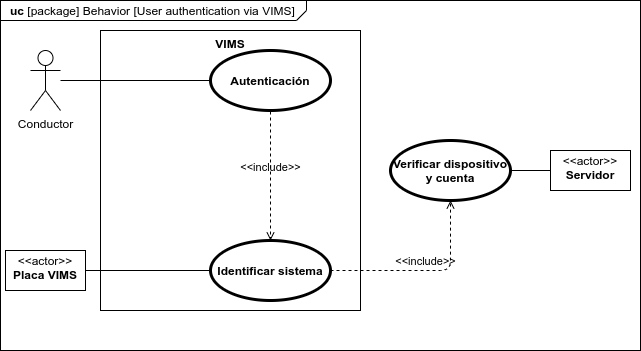
\includegraphics[width=\linewidth]{diagrams/UseCases-UC1 - auth.png}
  \caption{Caso de uso \texttt{01} -- \textit{autenticación}.}
  \label{uc:auth}
\end{figure}

\begin{table}[H]
  \centering
  \begin{tabularx}{\textwidth}{|c|c|X|}
    \hline
    \texttt{01}                                & \multicolumn{2}{c|}{\textit{Autenticación}}                                                                                                                                                                                                                 \\
    \hline
    \textbf{Descripción}                       & \multicolumn{2}{X|}{La placa identificará de forma inequívoca al conductor (usuario) y a sí misma frente al servidor.}                                                                                                                                      \\
    \hline
    \multirow{5}{*}{\textbf{Secuencia normal}} & \textbf{Paso}                                                                                                          & \textbf{Acción}                                                                                                                    \\
    \cline{2-3}
                                               & 1                                                                                                                      & \multicolumn{1}{L|}{El usuario se autentica contra la placa con su cuenta personal ya creada.}                                     \\
    \cline{2-3}
                                               & 2                                                                                                                      & \multicolumn{1}{L|}{La placa \ac{VIMS} recoge la información del usuario y la envía al servidor junto con su identificador único.} \\
    \cline{2-3}
                                               & 3                                                                                                                      & \multicolumn{1}{L|}{El servidor verifica que la cuenta del usuario existe y se asocia la información al dispositivo.}              \\
    \cline{2-3}
                                               & 4                                                                                                                      & \multicolumn{1}{L|}{La placa almacena la información del usuario y finaliza el proceso de inicio de sesión.}                       \\
    \hline
    \multirow{2}{*}{\textbf{Excepciones}}      & \textbf{Paso}                                                                                                          & \textbf{Acción}                                                                                                                    \\
    \cline{2-3}
                                               & 2 & \multicolumn{1}{L|}{La placa no cuenta con conexión a la red o el servidor no está disponible.} \\
    \cline{2-3}
                                               & 3                                                                                                                      & \multicolumn{1}{L|}{La cuenta del usuario no existe.}                                                                                                                                   \\
    \hline
  \end{tabularx}
\end{table}
